% !TEX root = ../my-thesis.tex
%
\chapter{Metodología}
\label{sec:methodology}

En esta sección revisamos el método propuesto para probar nuestra hipótesis junto a las consideraciones tomadas para su uso.
Las divisiones principales se enfocan en:\linebreak
(i) la preparación del modelo geométrico utilizado para la aproximación estructural y las propiedades bioelectromagnéticas de los tejidos incluidas las variaciones de conductividad, (ii) la solución del problema directo utilizando dipolos eléctricos que modelan puntos fijos de actividad neuronal equivalentes a respuestas evocadas (ER, del inglés \emph{evoked response}) y una representación matricial de las variaciones espacio-temporales de dicho dipolo, (iii) la solución del problema inverso de las señales simuladas para identificar la posición de las fuentes de actividad neuronal, y por último (iv) un análisis estadístico del estimador utilizando la frontera de Cramer-Rao para verificar su desempeño como estimador no sesgado.

\section{Método Propuesto}
\label{sec:methodology:method}

El objetivo es resolver el problema inverso y examinar el error asociado con el uso de distintos valores reportados de BSCR en diferentes áreas de actividad neuronal relacionadas con estímulos sensoriales \cite{McCann2019}.
Para ello, diseñamos un experimento que nos permitiría construir un estimador al implementar una solución del problema inverso con datos completamente simulados, y por ende con total control sobre las variables definidas como: la conductividad, la posición, orientación y magnitud de las fuentes de actividad neuronal, y el ruido añadido a las mediciones.
El proceso del experimento es una implementación completa de las soluciones a los problemas directo e inverso en el EEG con un posterior análisis estadístico. 
El problema directo nos permite obtener un modelo detallado de la actividad neuronal en la cabeza y simular mediciones de EEG con diferentes valores del BSCR.
En contraparte, el problema inverso resolverá las posiciones de las fuentes simuladas utilizando las mediciones generadas por el modelo del problema directo, y el análisis estadístico nos permitirá obtener la estimación de los valores de conductividad con base en el error incurrido en la localización de las fuentes de actividad neuronal respecto a su posición real agrupando por los distintos valores de conductividad utilizados, el esquema del experimento se presenta en la \cref{fig:methodology:pipeline}.

\begin{figure}[tb]
	\centering
	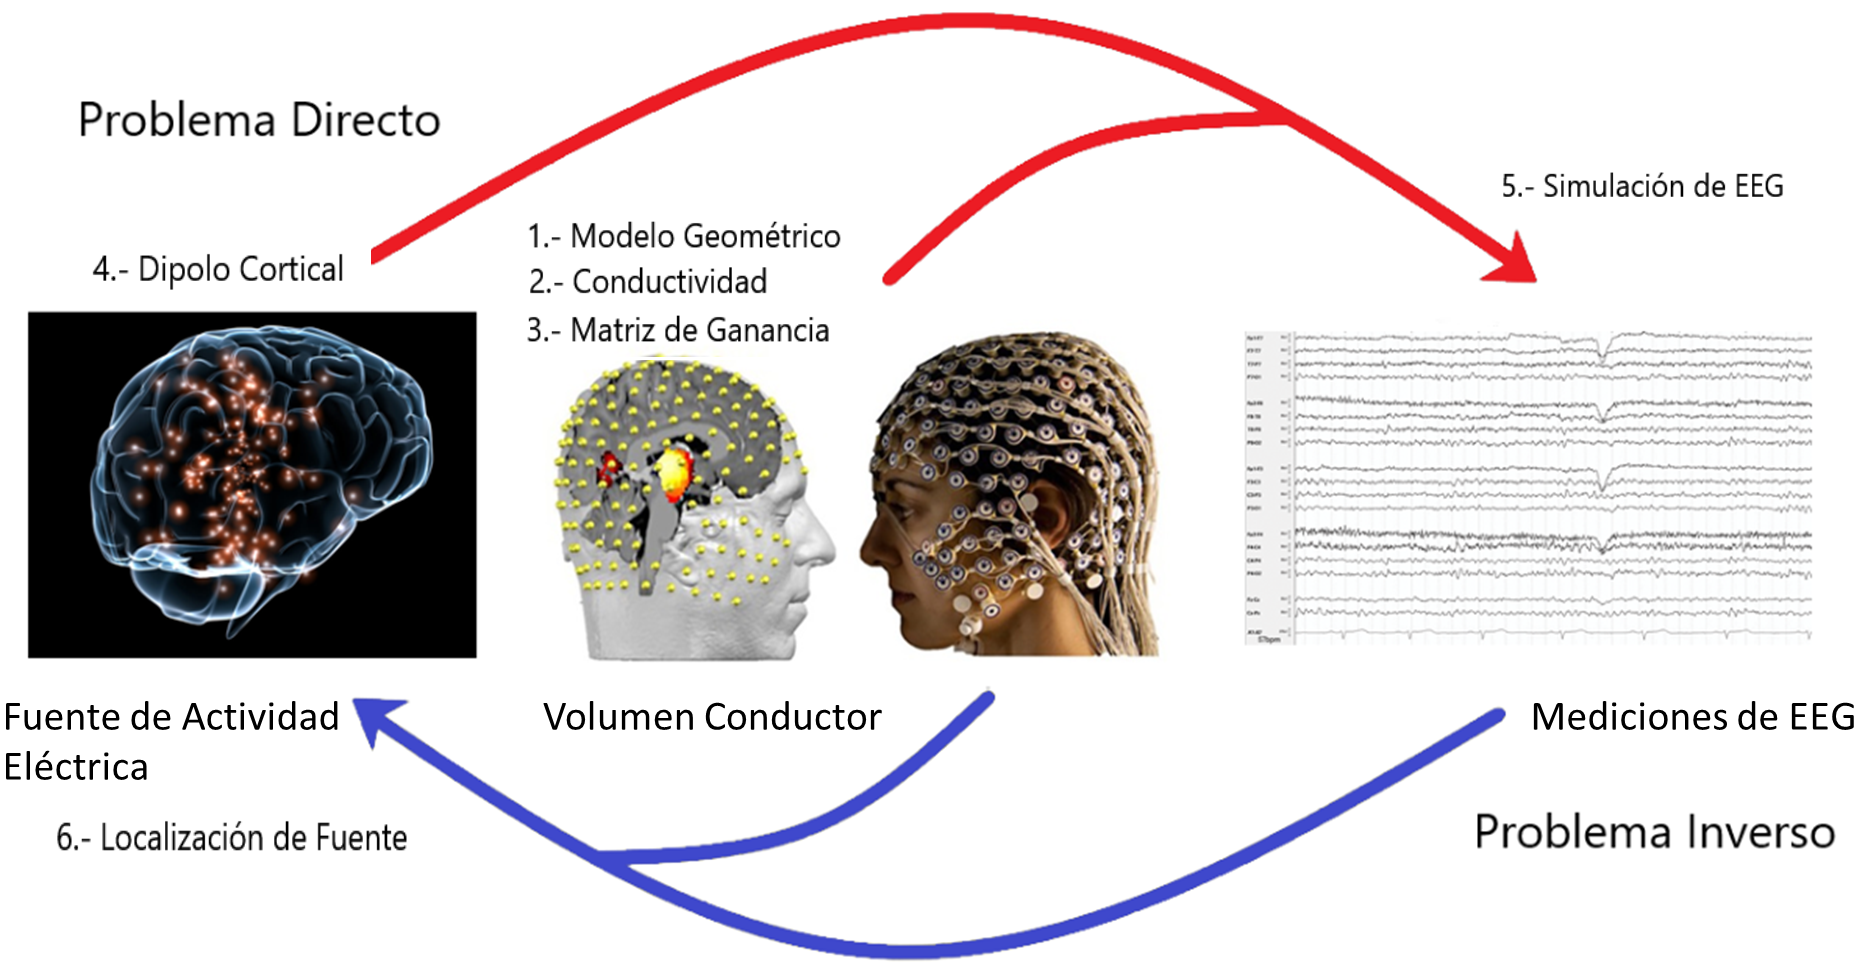
\includegraphics[width=\textwidth]{pipeline}
	\caption{Proceso del problema directo e inverso del EEG}
	\label{fig:methodology:pipeline}
\end{figure}

Basándonos en trabajo previo, decidimos resolver el problema inverso mediante filtrado espacial, en particular con el filtro propuesto en \cite{VanVeen1988}, el cual es catalogado como un método paramétrico, también conocido como ``método de dipolo de corriente equivalente''.
Como su nombre lo indica, estos métodos consisten en buscar en una serie predefinida de dipolos de corriente el que mejor se ajuste en su posición y orientación a las fuentes que generaron las mediciones de EEG  \cite{Hallez2007}.

Con el fin de realizar esta prueba de ajuste de los dipolos de corriente equivalente (solución del problema inverso) es necesario obtener la solución del problema directo. Existen varios métodos para obtener dicha solución \cite{Mosher1999}, de los cuales elegimos BEM para modelos geométricamente realistas \cite{Ermer2001}.
La razón de elegir este método radica en el precedente del uso de modelos con geometrías más sencillas en estudios similares \cite{Gutierrez2004}.
En la actualidad se cuenta con mayor facilidad de acceso a equipos de cómputo con el suficiente desempeño para obtener resultados en un tiempo razonable, esto aunado al desarrollo de métodos y software mucho más eficientes \cite{open,Clerc2010} nos presenta la posibilidad de implementar BEM para geometrías realistas como una evolución natural de los métodos utilizados anteriormente.

Una vez establecidos los métodos a utilizar en el método directo e inverso, se procedió a recopilar y formular la información necesaria para realizar los cálculos.
En el caso del problema directo los datos de entrada requeridos son: el modelo geométricamente realista que representará a los tejidos de la cabeza como un volumen conductor, una serie de dipolos que modelan el fenómeno de respuesta evocada, los valores a probar de la conductividad entre los tejidos, en específico la razón cerebro/cráneo, y por último el arreglo de sensores de EEG que medirán el campo eléctrico simulado.
Como resultado, se obtiene una matriz de ganancia dependiente de los valores de conductividad utilizados que dictamina como el arreglo de sensores de EEG captaría el campo eléctrico generado por las fuentes de actividad neuronal (dipolos) sobre la parte más superficial del modelo geométrico.

Para el problema inverso, los datos de entrada consisten en: las mediciones de EEG simuladas a partir de la solución del problema directo, el mismo modelo geométrico con su arreglo de EEG correspondiente, las matrices de ganancia generadas en el problema directo, y las propiedades pertinentes al método de filtrado espacial, como la matriz de covarianza de las mediciones y una matriz de covarianza del ruido.

Como resultado final de este método, obtenemos un kernel de proyección de las fuentes de actividad neuronal que el filtro espacial pudo localizar.
Lo que nos permite comparar la posición de los dipolos que fueron fijados en un principio en el problema directo contra la posición localizada por el filtro espacial con respecto a los diferentes valores de conductividad, y así obtener un estimador basado en los errores incurridos en la localización de estas fuentes.

\section{Construcción del Modelo Geométrico Realista}
\label{sec:methodology:model}

La construcción del modelo geométrico realista de los tejidos se basó en la plantilla ``Colin27 Average Brain 2008'' catalogada en \cite{Aubert-Broche2006}.
Esta consiste en una versión mejorada del modelo de original de Colin que resulta del promedio de 27 imágenes de resonancia magnética ponderadas en T1, T2, y densidad protónica, provenientes de diferentes mediciones del mismo sujeto \cite{Collins1998, Holmes1998}. 
Muestras de las imágenes de resonancia magnética de Colin27 se presentan en la \cref{fig:methodology:mri}.

\begin{figure}[tb]
	\centering
	\begin{subfigure}{0.49\textwidth}
		\centering
		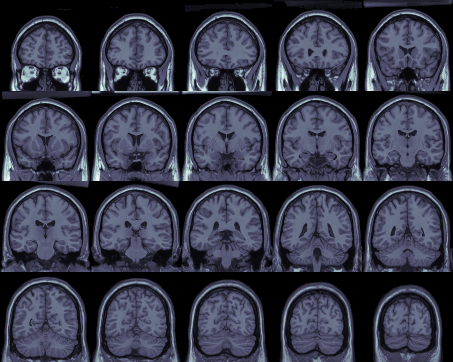
\includegraphics[width=\textwidth]{mri_coronal}
		\caption{Corte coronal}
		\label{fig:methodology:coronal}
		\vspace{0.1cm} % Add vertical space here
	\end{subfigure}
	\begin{subfigure}{0.49\textwidth}
		\centering
		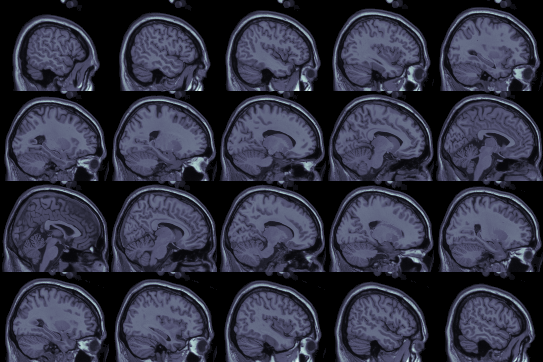
\includegraphics[width=\textwidth]{mri_sagital}
		\caption{Corte sagital}
		\label{fig:methodology:sagital}
		\vspace{0.1cm} % Add vertical space here
	\end{subfigure}
	\begin{subfigure}{0.49\textwidth}
		\centering
		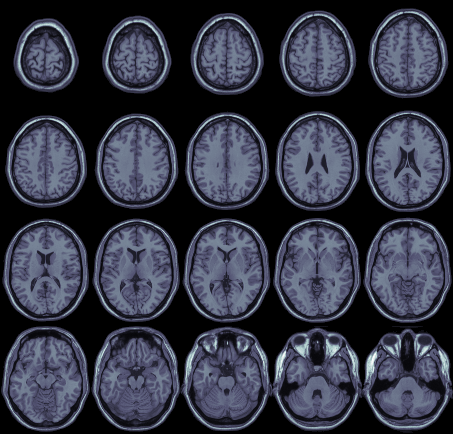
\includegraphics[width=\textwidth]{mri_axial}
		\caption{Corte axial}
		\label{fig:methodology:axial}
	\end{subfigure}
	\caption{Resonancia magnética de Colin27, tomada de \cite{Aubert-Broche2006}}
	\label{fig:methodology:mri}
\end{figure}

Con la información recopilada de la anatomía del sujeto se generó mediante el software libre Brainstorm \cite{brain2011} un conjunto de mallas teseladas y anidadas que representan las fases entre los diferentes tejidos de interés, esto es, cerebro, cráneo, y cuero cabelludo, presentadas en la \cref{fig:methodology:meshes}.
Debido al costo computacional del uso de BEM, la resolución de las mallas es diferente dependiendo de la profundidad de las fases, siendo cerebro/cráneo y cráneo/cuero cabelludo las que mayor resolución poseen (8640 triángulos y 4322 vértices para ambas), debido a que estas tienen una mayor sensibilidad al ser las más cercanas a la fuente de actividad neuronal y que representan por completo la capa de tejido óseo que servirá como volumen conductor, estas corresponden a las mallas de la \cref{fig:methodology:inner,fig:methodology:outer}.
Por estas razones es importante que ambas mallas tengan la misma resolución y no comprometan la precisión de los resultados. 

\begin{figure}[tbp]
	\centering
	\begin{subfigure}{0.45\textwidth}
		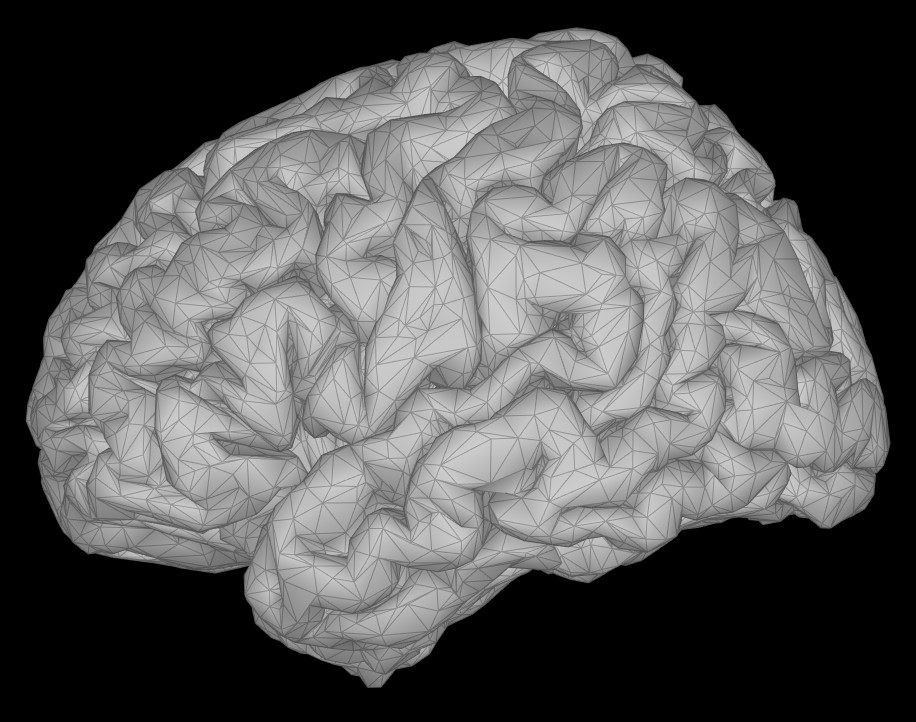
\includegraphics[width=\textwidth]{cortex}
		\caption{Corteza cerebral}
		\label{fig:methodology:cortex}
		\vspace{0.1cm}
	\end{subfigure}\hfill
	\begin{subfigure}{0.45\textwidth}
		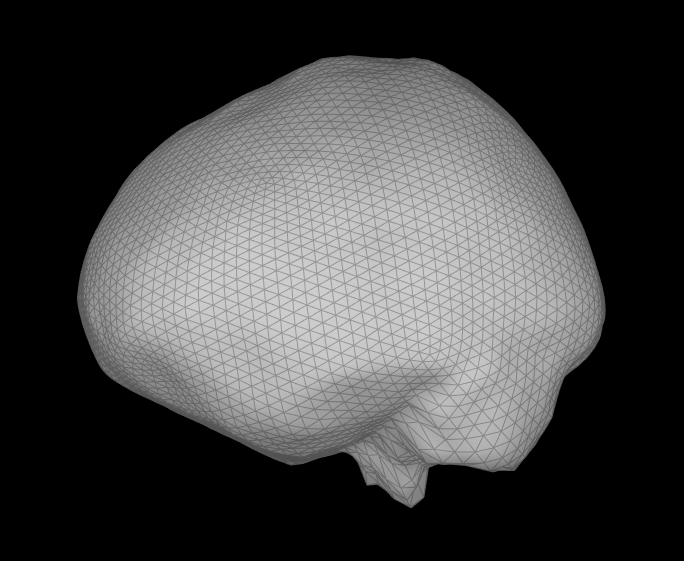
\includegraphics[width=\textwidth]{inner_skull}
		\caption{Capa interna del cráneo}
		\label{fig:methodology:inner}
		\vspace{0.1cm}
	\end{subfigure}\\
	\begin{subfigure}{0.45\textwidth}
		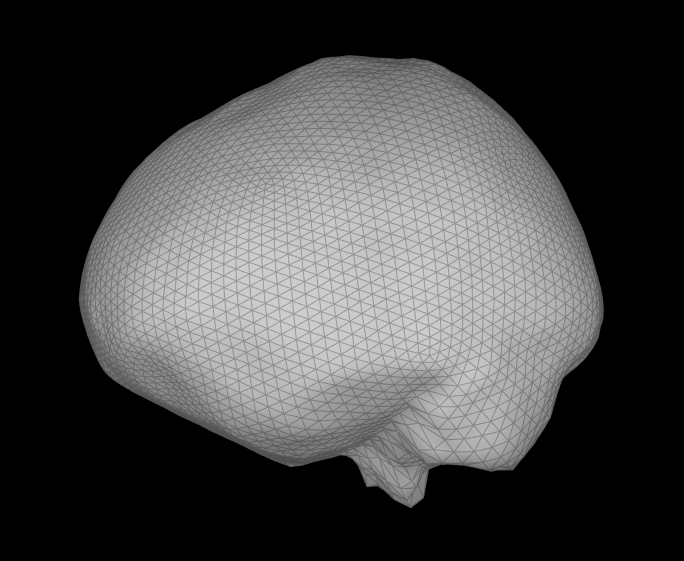
\includegraphics[width=\textwidth]{outer_skull}
		\caption{Capa externa del cráneo}
		\label{fig:methodology:outer}
	\end{subfigure}\hfill
	\begin{subfigure}{0.45\textwidth}
		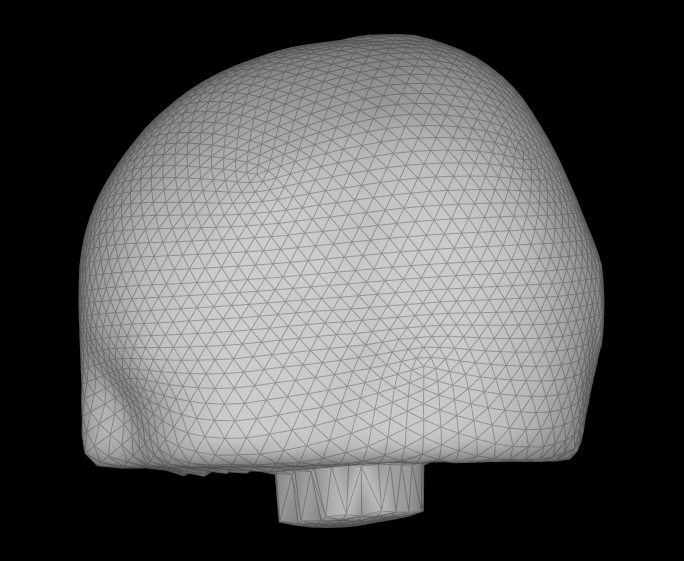
\includegraphics[width=\textwidth]{head}
		\caption{Cuero cabelludo}
		\label{fig:methodology:head}
	\end{subfigure}
	\caption{Mallas de las diferentes fases de los tejidos de la cabeza}
	\label{fig:methodology:meshes}
\end{figure}

La fase del cuero cabelludo/aire (mostrada en la \cref{fig:methodology:head}) tiene una resolución menor con 6480 triángulos y 3242 vértices.
Fue definida así porque corresponde al límite de resolución computable con la RAM de la estación de trabajo.
Aún así, es una resolución alta comparada con el uso recomendado del software \cite{tadelMEGEEGGroup2019a}.

Por último se tiene una malla que representa la corteza cerebral (\cref{fig:methodology:cortex}), la cual cuenta con una resolución de 29988 triángulos compuestos de 15002 vértices, los cuales tienen la finalidad de proporcionar ``dipolos elementales'' sobre los que se proyectarán los resultados. 
Esta malla es importante para el cálculo del campo eléctrico generado por actividad neuronal no influye drásticamente en el costo computacional y puede utilizarse una resolución mayor para representar con detalle los pliegues y concavidades de la corteza cerebral.
Todas las mallas en conjunto representan nuestro volumen conductor (mostrado en la \cref{fig:methodology:model}) sobre el que se implementarán los cálculos de BEM y la proyección del resultado del filtro espacial.

\begin{figure}[tbp]
	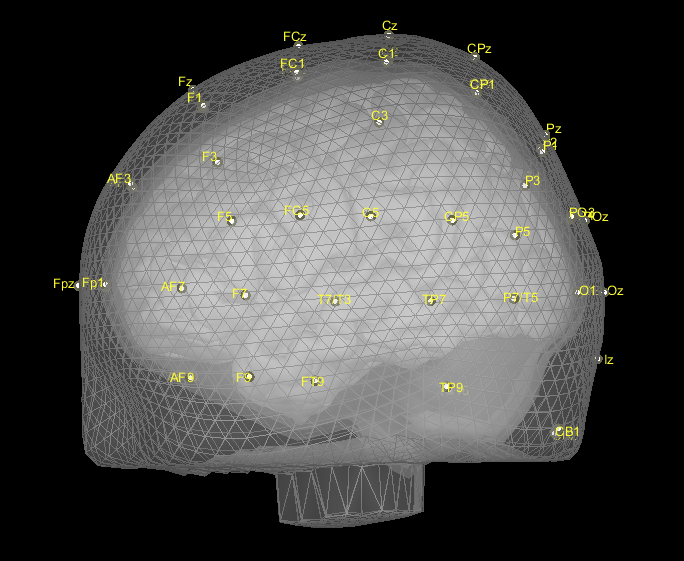
\includegraphics[width=\textwidth]{whole_model}
	\caption{Modelo geométricamente realista completamente anidado con sensores de EEG}
	\label{fig:methodology:model}
\end{figure}

\section{Variación de la Conductividad y Cálculo de la Matriz de Ganancia}
\label{sec:methodology:openmeeg}

La finalidad de resolver el problema inverso es ubicar la posición de la fuente de corriente que representa la actividad neuronal por lo que esta ubicación es la variable independiente al momento de hacer el cálculo, mientras que la conductividad se mantiene como un valor fijo.

En el área de neurociencias se suele mantener un valor nominal para la razón de conductividad cerebro-cráneo de 1:80 ($0.33\text{ S/m}$ para el cerebro y $0.0042 \text{ S/m}$ para el cráneo) \cite{Rush1968,Rush1969,Cohen1983}.
Sin embargo, múltiples estudios con diferentes acercamientos han publicado valores de la razón de conductividad cerebro-cráneo que se desvían significativamente del estándar de 1:80 \cite{McCann2019}.
Por esta razón, el objetivo de nuestro experimento es estimar el error incurrido en la localización de fuentes de actividad neuronal utilizando al BSCR como variable parámetro en la solución del problema inverso, mientras se toma por conocida la posición del dipolo de corriente y manteniéndose fija en todos los experimentos.

Regresando a \cref{lineal}, $L$ representa la llamada \emph{matriz de ganancia} que determina la sensibilidad del arreglo de electrodos en un EEG y como estos registrarán el campo eléctrico sobre el cuero cabelludo.
Para el cálculo de esta matriz de ganancia por medio de BEM se utilizó el software OpenMEEG \cite{open,open2}, donde las entradas fueron: nuestro modelo geométricamente realista, un arreglo de EEG con 65 sensores posicionados acorde al sistema internacional 10-10 (mostrado en la \cref{fig:EEG10-10}), y los valores de conductividad del cerebro, cráneo, y cuero cabelludo.
Se completó el cálculo de la matriz de ganancia para 10 valores del BSCR, presentados en la \cref{tab:bscr} de los cuales dos son valores aceptados en la literatura (1:20, 1:80) y los restantes se eligieron de \cite{McCann2019}.
El criterio para la elección de estos ocho valores fue que su estimación se realizó con métodos que involucraban el uso de EEG o EEG/MEG, esto con el fin de mantener relación con nuestra propia estimación y compararlos objetivamente.
La matriz de ganancia resultante de cada una de los valores del BSCR tiene $45006 \times 65$ elementos, que corresponden a los 65 canales del EEG y su respuesta a los 15002 vértices de la malla de la corteza cerebral del modelo geométrico en sus tres componentes vectoriales.

\begin{figure}[p]
	\centering
	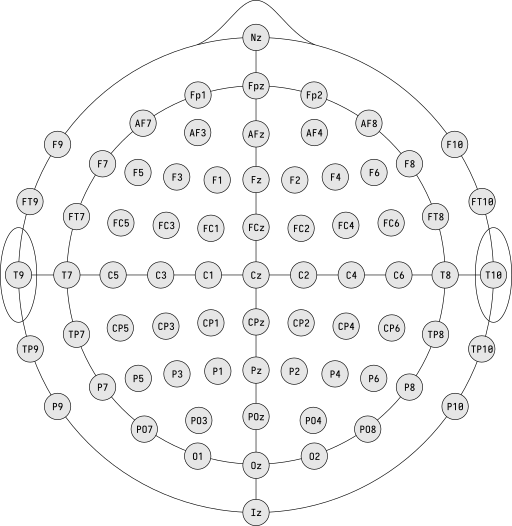
\includegraphics[width=0.75\textwidth]{EEG_10-10}
	\caption{Arreglo de electrodos EEG, tomada de \cite{krolEnglishEEGElectrode2020}.}
	\label{fig:EEG10-10}
\end{figure}

\begin{table}[p]
	\centering
	\begin{tabular}{@{}rrr@{}}
		\toprule
		ID & BSCR   & Referencias                                                                            \\ \midrule
		1  & 79.36  & \begin{tabular}[c]{@{}l@{}}\cite{Cohen1983}\end{tabular}                               \\
		2  & 208.33 & \begin{tabular}[c]{@{}l@{}}\cite{eriksenVivoHumanHead1990}\end{tabular}                \\
		3  & 68.96  & \begin{tabular}[c]{@{}l@{}}\cite{gonalvesVivoMeasurementBrain2003}\end{tabular}        \\
		4  & 22.17  & \begin{tabular}[c]{@{}l@{}}\cite{Baysal2004}\end{tabular}                              \\
		5  & 26.24  & \begin{tabular}[c]{@{}l@{}}\cite{Gutierrez2004}\end{tabular}                           \\
		6  & 41.84  & \begin{tabular}[c]{@{}l@{}}\cite{Dannhauer2011}\end{tabular}                           \\
		7  & 33.00  & \begin{tabular}[c]{@{}l@{}}\cite{aydinCombiningEEGMEG2014a}\end{tabular}               \\
		8  & 10.30  & \begin{tabular}[c]{@{}l@{}}\cite{acarHighresolutionEEGSource2016}\end{tabular}         \\
		9 & 20.00  & \begin{tabular}[c]{@{}l@{}}\cite{hoekemaMeasurementConductivitySkull2003}\end{tabular} \\
		10  & 80.00  & \begin{tabular}[c]{@{}l@{}}\cite{Rush1968}\end{tabular}                                \\ \bottomrule\\
	\end{tabular}
	\caption{Valores de la razón de conductividad cerebro-cráneo (BSCR) utilizados en el experimento.}
	\label{tab:bscr}
\end{table}

\section{Dipolos de corriente e implementación de la solución del problema directo}
\label{sec:methodology:direct_solved}

La matriz de ganancia de cada BSCR con el modelo geométrico completan el volumen conductor con sus propiedades electromagnéticas.
La pieza restante para el cálculo del problema directo es la fuente de actividad eléctrica que se propagará por dicho volumen conductor.
Como se había discutido anteriormente se decidió usar un dipolo eléctrico de posición fija gracias a que la actividad neuronal correspondiente a un ER se puede modelar como tal. 
Este dipolo varía su magnitud con el tiempo en un periodo de 600 ms, su función se observa en la \cref{fig:methodology:dipole}.
En cuanto a la posición, se decidió utilizar tres diferentes, cada una en distintas zonas del cerebro correspondientes a lugares de eventos de respuesta evocada, siendo estas: la corteza somatosensorial primaria (coordenadas MNI -52.2, -32.4, 55.8), corteza visual primaria (9.7, -98.6, 2.4), y corteza auditiva primaria (-65.0, -24.7, 11), estas posiciones se muestran en la \cref{fig:dipoles}.
Cabe mencionar que el sistema de coordenadas MNI es usualmente utilizado como referencia para la comparación de diferentes sujetos, pero el software utiliza para sus cálculos el sistema CTF/MRI al que denomina \emph{subject coordinate system} (SCS), por lo que toda futura mención de coordenadas corresponden a dicho sistema.

\begin{figure}[tb]
	\centering
	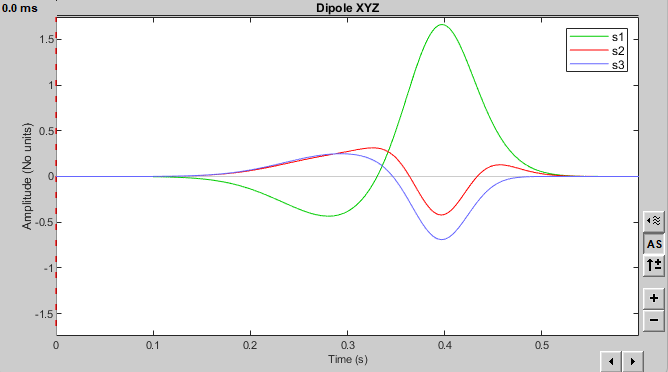
\includegraphics[width=\textwidth]{dipole-function}
	\caption{Función del dipolo eléctrico con respecto al tiempo. Dado que el dipolo es sintético, la amplitud no tiene unidades. Pero al momento de calcular el campo eléctrico generado por el dipolo, la magnitud se introduce en el cálculo con unidades de nAm.}
	\label{fig:methodology:dipole}
\end{figure}


\begin{figure}[tb]
	\centering
	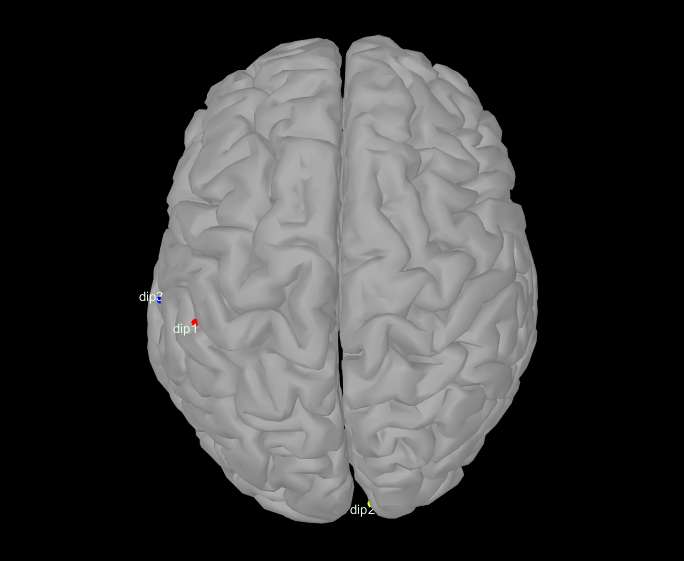
\includegraphics[width=\textwidth]{gfx/dipoles.png}
	\caption{Dipolos posicionados en la malla de la corteza cerebral, Dipolo 1 (rojo) corresponde a la zona somatosensorial, Dipolo 2 (amarillo) a la zona visual, y Dipolo 3 (azul) a la zona auditiva.}
	\label{fig:dipoles}
\end{figure}

Habiendo satisfecho los requisitos para la solución del problema directo este se calculó de la siguiente forma:

\begin{enumerate}
	\item Dentro del software Brainstorm, se crearon \emph{scouts} en la malla de la corteza cerebral. Estos consisten en las coordenadas SCS de las ROI. Estos fueron llamados \emph{dip1} (somatosensorial), \emph{dip2} (visual), y \emph{dip3} (auditiva).
	\item Los scouts fueron utilizados como dato de entrada en la solución del problema directo en Brainstorm junto con la función del dipolo con respecto al tiempo, el volumen conductor compuesto por el modelo geométricamente realista y la matriz de ganancia de cada BSCR importadas a Brainstorm, y por último el arreglo de sensores de EEG.
	\item Como resultado, obtuvimos 100 mediciones de EEG simuladas correspondientes a cada BSCR para cada uno de los tres scouts, siendo en total 300 mediciones de EEG.
	\item Tomando en cuenta de que estamos simulando nuestros datos y estamos en control de todas las variables, se procedió a añadir ruido en la implementación del problema directo para considerar otras condiciones de experimentos con pacientes. El ruido se añadió con una relación señal/ruido (SNR, del inglés \emph{signal-to-noise-ratio}) de 1\%, 5\%, y 10\% de la magnitud de las señales, usando una función de Brainstorm correspondiente a la ecuación: 
	\begin{equation}
		\label{eq:snr}
		\text{\emph{Source}} = \text{\emph{Source}} + \text{\emph{SNR}}\times(\text{\emph{randn}}(\text{\emph{size}}(\text{\emph{Source}})-0.5)) \times \text{\emph{max}}(\text{\emph{abs}}(\text{\emph{Source}}))\text{,}
	\end{equation}
	donde \emph{Source} es la señal de EEG simulada y SNR es la razón señal/ruido.
	\item De esta manera, obtuvimos 3 sets de 10,000 mediciones para cada uno de los 3 dipolos, sumando 90,000 mediciones simuladas de EEG diferentes.
\end{enumerate}

El proceso del problema directo se puede visualizar en la \cref{fig:methodology:direct_pipeline}.

\begin{figure}[!b]
    \centering
    \begin{tikzpicture}[node distance = 3.5cm, auto]
        % Define block styles
        \tikzstyle{block} = [rectangle, draw, fill=blue!20,
        text width=7em, text centered, rounded corners, minimum height=4em]
        \tikzstyle{line} = [draw, -{Latex}] % Use -{Latex} instead of -latex

        % Place nodes
        \node [block] (BEM) {Matriz de ganancia por cada BSCR, 10 en total};
        \node [block, right of=BEM] (PD) {Problema directo:\\100 simulaciones de EEG por cada matriz de ganancia: 1,000 en total};
        \node [block, right of=PD] (SNR) {Simulación con diferente SNR:\\3 niveles de SNR, 3,000 en total};
        \node [block, right of=SNR] (Sol) {Implementación para 3 zonas diferentes de la corteza cerebral:\\9,000 en total};
        
        % Add text on top of nodes
        \node at (BEM.north) [yshift=1em] {BEM con OpenMEEG};
        \node at (PD.north) [yshift=1em] {Implementando \cref{lineal} con Brainstorm};
        \node at (SNR.north) [yshift=1em] {Brainstorm};
        \node at (Sol.north) [yshift=1em] {Brainstorm};

        % Draw edges
        \path [line] (BEM) -- (PD);
        \path [line] (PD) -- (SNR);
        \path [line] (SNR) -- (Sol);
    \end{tikzpicture}
    \caption{Proceso del problema directo del EEG}
    \label{fig:methodology:direct_pipeline}
\end{figure}


\section{Implementación del Problema Inverso}
\label{sec:methodology:inverse_solved}

Dado que nuestra meta es estimar el error asociado con la resolución del problema inverso utilizando diferentes valores del BSCR en varias áreas de la corteza cerebral, implementamos la solución de la siguiente manera: emparejamos las 100 mediciones de EEG resultantes de cada BSCR (1,000 en total) con cada una de las 10 matrices de ganancia de los diferentes BSCR a probar, lo que resulta en 10,000 combinaciones distintas para un solo dipolo y nivel de ruido.
Teniendo 3 niveles de ruido y 3 dipolos diferentes, se obtiene un total de 90,000 combinaciones distintas y, por ende, el mismo número de implementaciones del problema inverso a resolver, como se muestra en la \cref{fig:methodology:inverse_pipeline}.

\begin{figure}[tb]
	\centering
	\begin{tikzpicture}[node distance = 3.5cm, auto]
		% Define block styles
		\tikzstyle{block} = [rectangle, draw, fill=blue!20,
		text width=7em, text centered, rounded corners, minimum height=4em]
		\tikzstyle{line} = [draw, -{Latex}] % Use -{Latex} instead of -latex

		% Place nodes
		\node [block] (1) {100 mediciones de EEG de un BSCR contra las 10 matrices de ganacia diferentes:\\1,000 en total};
		\node [block, right of=1] (2) {Expansión de cada set de mediciones de EEG por BSCR con cada matriz de ganancia:\\10,000 en total};
		\node [block, right of=2] (3) {Simulación con los 3 niveles de SNR:\\30,000 en total};
		\node [block, right of=3] (4) {Implementación para 3 zonas diferentes de la corteza cerebral:\\90,000 en total};

        % % Add text on top of nodes
        % \node at (1.north) [yshift=1em] {Brainstorm};
        % \node at (2.north) [yshift=1em] {Brainstorm};
        % \node at (3.north) [yshift=1em] {Brainstorm};
        % \node at (4.north) [yshift=1em] {LCMV en Brainstorm};

		% Draw edges
		\path [line] (1) -- (2);
		\path [line] (2) -- (3);
		\path [line] (3) -- (4);
	\end{tikzpicture}
	\caption{Pareamiento de mediciones de EEG con las matrices de ganancia para el problema inverso del EEG}
	\label{fig:methodology:inverse_pipeline}
\end{figure}

Al igual que en el cálculo del problema directo, se utilizó la suite Brainstorm en Matlab para el cómputo de los 90,000 conjuntos de datos.
Específicamente, las librerías pertinentes para el procesado de las mediciones de EEG fueron extraídas y modificadas para manejar de forma óptima el procesamiento de nuestro gran volumen de información mediante automatización y combinación de procesamientos posteriores.
La razón de utilizar Brainstorm para resolver el problema inverso es que dentro de las opciones de métodos de solución incluidas se encuentra una variación del método de filtrado espacial LCMV \cite{Jaiswal2020}.
Este método de filtrado espacial es de interés para el laboratorio por su versatilidad, y ha sido utilizado anteriormente en proyectos relacionados \cite{jimenez-cruzReducedrankBeamformingBrain2019, Jimenez-Cruz2023}.

La implementación del filtro espacial LCMV en Brainstorm obtiene mapas del pseudo-índice de actividad neuronal (PNAI, del inglés \emph{pseudo neuronal activity index}), denominado así por las modificaciones introducidas en \cite{Jaiswal2020} a la definición del índice de actividad neuronal del filtro LCMV original en \cite{VanVeen1997}.
Estas modificaciones consisten en el uso exclusivo de la matriz de covarianza de las mediciones de EEG para la normalización de los mapas de actividad neuronal, dejando de lado la matriz de covarianza del ruido de las mediciones de la definición original.

La opción elegida de ejecución de este método de filtrado espacial sobre una medición de EEG resulta en el cálculo de un kernel de proyección del campo eléctrico detectado.
Este kernel reconstruye, localiza y visualiza las fuentes de actividad neuronal en forma de mapas del PNAI sobre la serie de dipolos que componen la malla de la corteza cerebral, así como su propagación a través de las otras mallas que constituyen el modelo geométrico.
Este kernel corresponde al definido por \cref{beamformer4} con la diferencia de que la matriz de covarianza del ruido no es utilizada en el cálculo y se define como una matriz identidad.

Tomando en cuenta que tenemos 90,000 combinaciones de mediciones de EEG y matrices de ganancia, debería de obtenerse un kernel de proyección para cada una de estas combinaciones.
Sin embargo, dado que el filtro espacial tiene como datos de entrada las mediciones de EEG, la matriz de ganancia, y la matriz de covarianza, esta última puede ser calculada a partir de las 100 mediciones de EEG de cada BSCR, obteniendo un kernel de mayor precisión que puede ser calculado para cada una de esas 100 mediciones de EEG en cualquier momento. 
De esta manera se reduce el número de archivos necesarios y el espacio ocupado en el disco del equipo de cómputo.
Esta fue una de las razones de realizar 100 simulaciones de EEG para cada combinación de dipolos y BSCR durante el proceso del problema directo: mejorar la robustez del estimador y evitar sesgos durante el análisis del problema inverso.
En total se obtuvieron 900 kernels de proyección, 100 por cada BSCR, para cada uno de los tres dipolos y tres niveles de SNR.
Esto nos asegura tener una muestra suficiente para observar la variabilidad de los resultados al utilizar valores distintos de BSCR con el que fueron simuladas las mediciones de EEG, permitiéndonos medir el error de localización de las fuentes de actividad neuronal.

\section{Error de Localización de las Fuentes de Actividad Neuronal}
\label{sec:methodology:estimator}

Para la cuantización del error de localización se procedió obtener la posición de magnitud máxima de los mapas de PNAI generados por el kernel de proyección para cada uno de los 90,000 conjuntos de datos. 
Estos fueron separados y analizados por cada BSCR, dipolo, y nivel de SNR.

La posición de magnitud máxima fue obtenida al implementar el kernel de proyección correspondiente a las mediciones de EEG en el instante $t=$ 397.2 ms, el cual es en el que se encuentra la magnitud máxima de la función del dipolo con respecto al tiempo.
Con el fin de mejorar la precisión de la localización de la magnitud máxima, se limitó el área sobre la cual se buscó el punto máximo en el mapa de PNAI, siendo tres diferentes áreas de búsqueda, una para cada uno de los distintos dipolos, siendo estas de 29.17 cm$^2$ para el Dipolo 1 (correspondiendo al área de la zona somatosensorial), 51.75 cm$^2$ para el Dipolo 2 (correspondiente al área visual primaria), y 76.92 cm$^2$ para el Dipolo 3 (correspondiente al área auditiva primaria), como se muestra en la \cref{fig:dipoles-zones}.
Cabe mencionar que las áreas de búsqueda se apegan a los pliegues y concavidades de la malla de la corteza cerebral, elevando el tamaño de las áreas de búsqueda y permitiendo la localización de la magnitud máxima dentro de estos pliegues.

\begin{figure}[tb]
\centering
    \begin{subfigure}[t]{0.49\textwidth}
        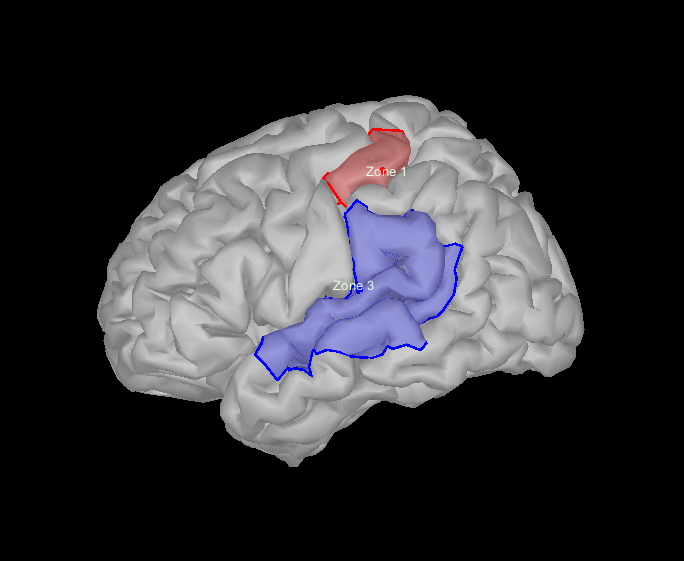
\includegraphics[width=\textwidth]{gfx/zone_1-2.png}
        \caption{Zonas de búsqueda de actividad neuronal en el problema inverso correspondientes a las zonas somatosensorial y auditiva de las zonas de Brodmann.}
        \label{fig:zone1-2}
    \end{subfigure}
	\hfill
    \begin{subfigure}[t]{0.49\textwidth}
        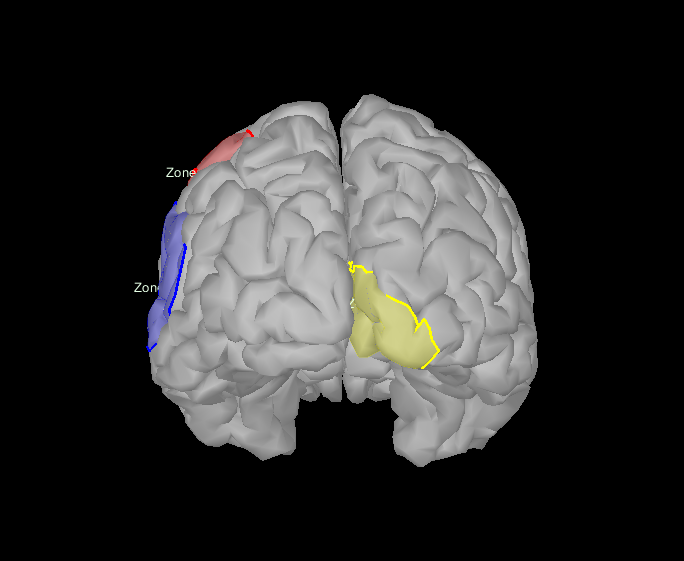
\includegraphics[width=\textwidth]{gfx/zone_3.png}
        \caption{Zona de búsqueda 3 correspondiente a la zona visual de las zonas de Brodmann.}
        \label{fig:zone3}
    \end{subfigure}
    \caption{Zonas de busqueda en la solución del problema inverso.}
    \label{fig:dipoles-zones}
\end{figure}

Las posiciones de magnitud máxima de cada medición de EEG, correspondientes a sus respectivas áreas de búsqueda, fueron obtenidas en coordenadas SCS y agrupadas en sus respectivos dipolos, valor de BSCR, y niveles de SNR, obteniendo como resultado 900 conjuntos de 100 posiciones de magnitud máxima. 
Al explorar la distribución de las posiciones de magnitud máxima se observó que estas no se distribuían normalmente.
Como era de esperarse, la distribución de los resultados en general tenía una tendencia natural a 0, lo que generaba una distribución sesgada a la derecha, por lo que se decidió utilizar la media del percentil P$_{95}$ como el estimador de la posición de magnitud máxima, y la distancia Euclidiana entre la posición real y la posición de magnitud máxima como el estimador del error de localización.
Una vez obtenidos los estimadores de la posición de magnitud máxima y el error de localización, se procedió a estandarizar el error de localización con respecto a la resolución de la malla de la corteza cerebral utilizando la distancia media y la desviación estándar entre los vértices de los triángulos de la malla de la corteza cerebral.
Por lo tanto, los estimadores de la posición de magnitud máxima y el error de localización se definieron como:
\begin{equation}
	\label{eq:mean_error}
	\text{Error}_{\text{estandarizado}} = \frac{\text{Posición}_{\text{localización}}-\text{Posición}_{\text{real}}}{\text{Distancia media}_{\text{vértices}}}\text{,}
\end{equation}
para el la estandarización del error de localización, y
\begin{equation}
	\label{eq:sd_error}
	\text{Desviación estándar}_{\text{estandarizada}} = \frac{\text{Desviación estándar}_{\text{localización}}}{\text{Distancia media}_{\text{vértices}}}\text{,}
\end{equation}
para la desviación estándar del error de localización.

\section{Análisis Estadístico Propuesto}
\label{sec:methodology:cbr-analysis}

Para determinar el desempeño del estimador se utilizó la CRB, la cual proporciona un límite inferior en la varianza de los errores en la estimación de parámetros no sesgados.
La CRB tiene la característica de ser universal, es decir, independiente del algoritmo utilizado para estimadores no sesgados, y asintóticamente ajustado, lo que significa que para ciertas distribuciones, existen algoritmos que alcanzan el límite a medida que el número de muestras aumenta \cite{Muravchik1999, Escalona-Vargas2013}.
Esta última característica es de particular interés para nuestro proyecto, y una razón más para realizar las 100 simulaciones de EEG para cada combinación de dipolos, valor de BSCR, y nivel de SNR durante el proceso del problema directo.

Este límite teórico inferior de la varianza del error para un estimador no sesgado se representa como una desigualdad con el valor esperado del estimador de la forma:
\begin{equation}
	\label{eq:crb2}
	\text{E}\left\{(\hat{\theta} - \theta)(\hat{\theta} - \theta)^{\text{T}}\right\} \geq \text{CRB}(\theta)\text{,}
\end{equation}
donde ${\theta}$ representa el parámetro de interés (la posición del dipolo en nuestro caso) y $\hat{\theta}$ es un estimador no sesgado del valor de $\theta$. A su vez, la varianza de cualquier estimador no sesgado $\hat{\theta}$ de $\theta$ está acotada por la inversa de la matriz de información de Fisher, la cual se define como:
\begin{equation}
	\label{eq:crb}
	\text{CRB}(\theta) = \left[\mathcal{I}(\theta)\right]^{-1}\text{,}
\end{equation} 
que en nuestro caso está dada como la inversa de la matriz de información correspondiente al EEG
\begin{equation}
	\label{eq:crbj}
	\text{CRB}(\theta) = [J^{\text{EEG}}(\theta)]^{-1}\text{,}
\end{equation} 
siendo la matriz de información de Fisher para el EEG
\begin{equation}
	\label{eq:fisher}
	J_{ij}^{\text{EEG}}(\theta) = q^{\text{T}}\left(\pdv{k}{\theta_{i}}\right)^{\text{T}}\frac{\text{L}^{\text{T}}\text{L}}{\sigma^2_{\text{E}}}\left(\pdv{k}{\theta_{i}}\right)q\text{,}
\end{equation}
donde $q$ es la magnitud del dipolo en el instante de 397.2 ms, $\text{L}$ es la matriz de ganancia, $\sigma^2_{\text{E}}$ es la varianza del ruido de las mediciones de EEG, y $\pdv{k}{\theta_{i}}$ es la derivada parcial de las posiciones de los dipolos con respecto a la posición de los sensores de EEG \cite{nielsenCramerRaoLowerBound2013, Stoica1988, Muravchik1999}. 

Este análisis estadístico se realizó con cada matriz de ganancia de los 10 BSCR, para cada uno de los tres dipolos, y para cada uno de los tres niveles de SNR. 
Dando como resultado en 90 valores de CRB. 
Este proceso, junto con la estimación del error incurrido en la localización de fuentes de actividad neuronal, se puede visualizar en la \cref{fig:methodology:statistical_pipeline}.

\begin{figure}[tbp]
	\centering
	\begin{tikzpicture}[node distance = 3.5cm, auto]
		% Define block styles
		\tikzstyle{block} = [rectangle, draw, fill=blue!20,
		text width=7em, text centered, rounded corners, minimum height=4em]
		\tikzstyle{line} = [draw, -{Latex}] % Use -{Latex} instead of -latex

		% Place nodes
		\node [block] (1) {Ejecución del kernel de proyección para cada medición de EEG en el instante de 397.2 ms};
		\node [block, right of=1] (2) {Obtención de la posición de magnitud máxima local};
		\node [block, right of=1] (2) {Estimador de la posición de magnitud máxima y el error de localización};
		\node [block, right of=2] (3) {Estandarización del error de localización con respecto a la resolución de la malla de la corteza cerebral};
		\node [block, right of=3] (4) {Análisis estadístico del estimador con la frontera de Cramér-Rao};
		% Draw edges
		\path [line] (1) -- (2);
		\path [line] (2) -- (3);
		\path [line] (3) -- (4);
	\end{tikzpicture}
	\caption{Proceso del análisis estadístico del estimador}
	\label{fig:methodology:statistical_pipeline}
\end{figure}